\chapter{Beispielapp - Computer Museum Guide}

\section{App Beschreibung}
Als Beispielapp haben wir einen Guide f�r ein Computer Museum entworfen. Der Guide zeigt Informationen zu den ausgestellten Computern und beinhaltet eine Karte des Museums �ber welche ebenfalls auf die Informationen �ber die ausgestellten Computer zugegriffen werden kann. Zus�tzlich k�nnen Informationen zum Museum abgerufen werden.

\section{Einrichtung}
Im CMS haben wir ein neues Dokument erstellt und als Start-Artikel die Einstiegsseite hinterlegt. Die n�tigenField Types und Templates haben wir in der Datenbank hinterlegt.

\subsection{Field Types}
Wir haben folgende \emph{Field\_types} definiert:

\begin{tabular}{|l|l|}
\hline 
\textbf{Name} & \textbf{Beschreibung} \\ 
\hline 
text & normaler Text \\ 
\hline 
html\_text & HTML Text welcher entsprechend verarbeitet wird \\ 
\hline 
resource\_path & Pfadangabe f�r verlinkte Dateien (Bilder, Videos, etc.) \\ 
\hline 
link\_to\_article & Link zu einem Anderen Artikel \\ 
\hline 
url & URL \\ 
\hline 
number & Zahl \\ 
\hline 
color & Farbe \\ 
\hline 
\end{tabular} 
\\
\\
\\
\textbf{Hinweis:} Mit \emph{html\_text} haben wir uns eine Art Joker-Feld geschaffen. Wir k�nnen damit beliebigen HTML Code durch die App verarbeiten lassen und k�nnen so auch Javascript nutzen. Dies erm�glicht uns, in der App gewisse Logik auszuf�hren oder Sachen darzustellen welche nicht durch ein implementiertes Template abgedeckt werden.

\newpage
\subsection{Templates}
Folgende \emph{einfachen Templates} und emph{Composite Templates} haben wir definiert.

\subsubsection{Einfache Templates}

\begin{itemize}

\item \textbf{Main Menu Item} (Hauptmen�punkt): \\
Felder: \\
\begin{tabular}{|l|l|l|}
\hline
\textbf{Name} & \textbf{Beschreibung} & \textbf{Field\_Type} \\
\hline
Label & Beschriftung & text \\
\hline
Article Link & Link zum Artikel & link\_to\_article \\
\hline
Background Color & Hintergrundfarbe & color \\
\hline
Button Image Normal & Link zum "Button Bild" & resource\_path \\
\hline
Button Image Pressed & Link zum "Button gedr�ckt Bild" & resource\_path \\
\hline
\end{tabular}

\item \textbf{Tabbar Item} (Tabbar Eintrag): \\
Felder: \\
\begin{tabular}{|l|l|l|}
\hline
\textbf{Name} & \textbf{Beschreibung} & \textbf{Field\_Type} \\
\hline
Icon & Link zum Bild & resource\_path \\
\hline
Label & Beschriftung & text \\
\hline
Link to Article & Verlinkter Artikel & link\_to\_article \\
\hline
\end{tabular}

\item \textbf{Image} (Bild): \\
Felder: \\
\begin{tabular}{|l|l|l|}
\hline
\textbf{Name} & \textbf{Beschreibung} & \textbf{Field\_Type} \\
\hline
Title & �berschrift & text \\
\hline
Image & Link zum Bild & resource\_path \\
\hline
\end{tabular}

\item \textbf{Location} (Ort): \\
Felder: \\
\begin{tabular}{|l|l|l|}
\hline
\textbf{Name} & \textbf{Beschreibung} & \textbf{Field\_Type} \\
\hline
Label & Beschriftung & text \\
\hline
Article Link & Link zum Artikel & link\_to\_article \\
\hline
X Coordinate & X Koordinaten im Bild & number \\
\hline
Y Coordinate & Y Koordinaten im Bild & number \\
\hline
Pin Icon & Link zum Icon & resource\_path \\
\hline
\end{tabular}

\item \textbf{Computer Info Page} (Informationen �ber einen Computer): \\
Felder: \\
\begin{tabular}{|l|l|l|}
\hline
\textbf{Name} & \textbf{Beschreibung} & \textbf{Field\_Type} \\
\hline
Title & �berschrift & text \\
\hline
Main Image & Bild des Computers & resource\_path \\
\hline
Image Source & Quellenangabe & text \\
\hline
Computer Info Text & Beschreibung & text \\
\hline
\end{tabular}

\item \textbf{HTML Page} (HTML Seite): \\
Felder: \\
\begin{tabular}{|l|l|l|}
\hline
\textbf{Name} & \textbf{Beschreibung} & \textbf{Field\_Type} \\
\hline
HTML Text & HTML Code der angezeigt wird & html\_text \\
\hline
\end{tabular}



\end{itemize}



\subsubsection{Composite Templates}

\begin{itemize}

\item \textbf{Main Menu} (Hauptmen�): \\
Felder: \\
\begin{tabular}{|l|l|l|}
\hline
\textbf{Name} & \textbf{Beschreibung} & \textbf{Field\_Type / Template} \\
\hline
Title & �berschrift & text \\
\hline
Menu Item 1 & 1. Men�punkt (ZZ Spectrum) & Main Menu Item \\
\hline
Menu Item 1 & 2. Men�punkt (Commodore 64) & Main Menu Item \\
\hline
Menu Item 1 & 3. Men�punkt (Lilith Computer) & Main Menu Item \\
\hline
Menu Item 1 & 4. Men�punkt (Commodore Amiga 500) & Main Menu Item \\
\hline
\end{tabular}

\item \textbf{Tabbar} (Tabbar, welche ausser auf dem Startbildschirm immer angezeigt wird): \\
Felder: \\
\begin{tabular}{|l|l|l|}
\hline
\textbf{Name} & \textbf{Beschreibung} & \textbf{Field\_Type / Template} \\
\hline
Tabbar Item 1 & 1. Tabbar Item (Computers) & Main Menu Item \\
\hline
Tabbar Item 1 & 2. Men�punkt (Karte) & Main Menu Item \\
\hline
Tabbar Item 1 & 3. Men�punkt (Info) & Main Menu Item \\
\hline
\end{tabular}

\item \textbf{Computer Museum Map View} (Museumskarte): \\
Felder: \\
\begin{tabular}{|l|l|l|}
\hline
\textbf{Name} & \textbf{Beschreibung} & \textbf{Field\_Type / Template} \\
\hline
Title & �berschrift & text \\
\hline
Map Image & Karte & resource\_path \\
\hline
ZX Spectrum Location & Koord. zum ZX Spectrum & Location \\
\hline
C64 Location & Koord. zum C64 & Location \\
\hline
Lilith Computer Location & Koord. zum Lilith & Location \\
\hline
\end{tabular}

\end{itemize}

\newpage
\section{Look and Feel}
In der Beispielapp sind einige wenige Views implementiert welche die Nutzung der \emph{Templates} veranschaulichen. \\
\\
\textbf{Start View} \\
Die Start View wird beim �ffnen der App angezeigt. Das einzige genutzte Template ist ein \emph{Image} mit dem Logo der App und dem Link auf die Main Menu View.\\
\\
\textbf{Main Menu View} \\
Das Composite Template \emph{Main Menu} wird genutzt um auf die einzelnen Info Views zu referenzieren und das Template \emph{Tabbar} wird f�r das schnelle Wechseln zwischen den Kategorien genutzt.\\
\\
\textbf{Map View} \\
Die Karte des Museums wird als Bild mit dem Composite Template \emph{Computer Museum Map View} umgesetzt und die Links zu den Computerinformationen sind \emph{Locations}. \\
\\
\textbf{Info View}
Die Info View zeigt die genauen Informationen eines Computers an. Wir haben daf�r das Template \emph{Computer Info Page} genutzt.



\begin{figure}[H]
	\centering
	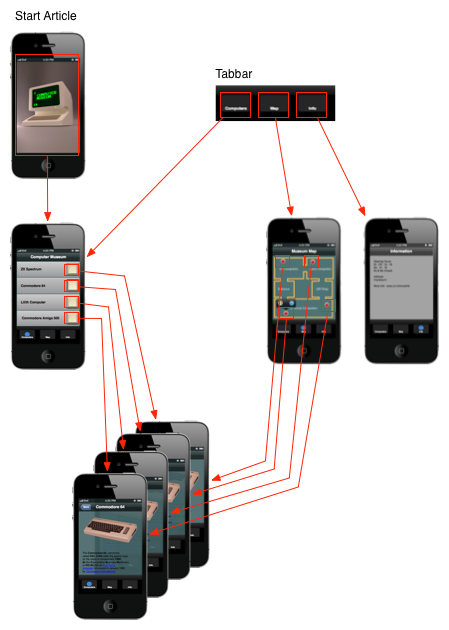
\includegraphics[scale=0.37]{graphics/app/userflow.png}
	\caption{\textbf{Look and Feel} }
	\label{lookAndFeel}
\end{figure}

In \autoref{lookAndFeel} sieht man wie einzelenen Views aussehen und wie die Artikel untereinander referenziert sind um die Navigation zu erm�glichen.